\chapter{Implementation}

\label{ch:implementation}

%
%
%
%
%
\section{Dimensionality Reduction}

Machine learning with high-dimensional data, such as images, is often computationally intensive. Atari 2600 frames are RGB images ($3$ channels) of size $210 \times 160$, expressed in shorthand as $(3, 210, 160)$. (This data is much higher in dimensionality than MNIST, which has dimensions $(1, 28, 28)$). Considering the training sets considered in this project are of hundreds of thousands of images, data points of dimension $(3, 210, 160)$ are too computationally intensive with the best hardware available (2 $\times$ NVIDIA Tesla K80 GPU Accelerators). It is therefore necessary to reduce the dimensionality of our data set. Google DeepMind's \textit{Human-level Control Through Deep Reinforcement Learning} \cite{Mnih2015} made use of Stella, as we have, and have convincingly struck a reasonable balance between resolution and dimensionality reduction. This section will be a short but necessary mentioning of the pre-processing pipeline used to generate the data sets in later chapters.

\subsection{Pre-processing Pipeline}

\subsubsection{Ensuring Object Persistence}
Atari 2600 games can only store a limited number of sprites per frame due to the limitations in hardware during its development \cite{Mnih2015}. This is an issue as some objects that appear in one frame fail to appear in the next. To solve this lack of object persistence, even and odd frames are combined by taking the maximum over each channel (RGB). By taking the maximum, we ensure that any object present in one frame is also present in the other. 

\begin{figure*}
\centering
\captionsetup{justification=centering}
\begin{multicols}{3}
    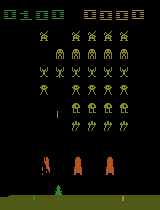
\includegraphics[scale=0.8]{figures/related_work/space_invaders_341_rgb_even.png}\par 
    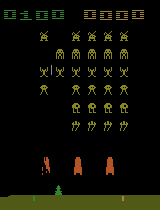
\includegraphics[scale=0.8]{figures/related_work/space_invaders_341_rgb_odd.png}\par
    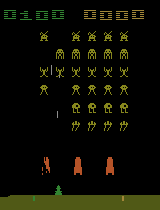
\includegraphics[scale=0.8]{figures/related_work/space_invaders_341_rgb_maximum_of_even_odd.png}\par    
    \end{multicols}
\begin{multicols}{3}
    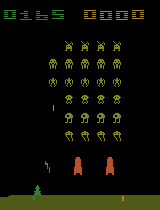
\includegraphics[scale=0.8]{figures/related_work/space_invaders_831_rgb_even.png}\par
    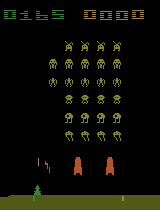
\includegraphics[scale=0.8]{figures/related_work/space_invaders_831_rgb_odd.png}\par
    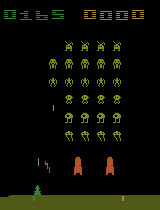
\includegraphics[scale=0.8]{figures/related_work/space_invaders_831_rgb_maximum_of_even_odd.png}\par
\end{multicols}
\begin{multicols}{3}
    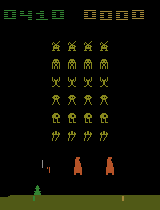
\includegraphics[scale=0.8]{figures/related_work/space_invaders_1044_rgb_even.png}\par
    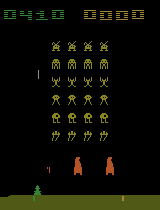
\includegraphics[scale=0.8]{figures/related_work/space_invaders_1044_rgb_odd.png}\par
    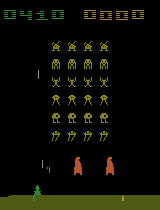
\includegraphics[scale=0.8]{figures/related_work/space_invaders_1044_rgb_maximum_of_even_odd.png}\par
\end{multicols}
\caption{A collection of frames captured from Space Invaders emulated on Stella. \textbf{Left column:} an even frame. \textbf{Middle column:} the (odd) frame following. \textbf{Right column:} Combining the even and odd frames by taking the maximal value over each channel (RGB). Clearly the bullets visible in one frame fail to persist in the next. As mentioned, this is due to the limited number of sprites Atari 2600 can load in a single frame.}
\label{fig:even_and_odd_frames_space_invaders}
\end{figure*}

\subsubsection{Extracting Luminance and Cropping}
The luminance $Y$ is then extracted from the RGB image \cite{Stokes1996}:
\begin{align}
Y = 0.2126\times R + 0.7152\times G + 0.0722\times B
\end{align}
The resultant greyscale image of shape $(1, 210, 160)$ is cropped to $(1, 84, 84)$.

\subsubsection{File Formats}
Image formats were discovered to be more important than originally thought. Empirically, PNG or GIF formats were reasonable formats, but using JPEG often resulted in distortions near the perimeter of objects. An example of this effect is shown in Figure (\ref{fig:pong_729_pre_processed}).\\

\begin{figure}[h!]
\centering
\captionsetup{justification=centering}
\begin{multicols}{1}
    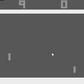
\includegraphics[scale=2.0]{figures/related_work/pong_729_pre_processed.jpeg}\par
    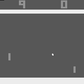
\includegraphics[scale=2.0]{figures/related_work/pong_729_pre_processed.png}\par
\end{multicols}
\caption{Pre-processed frames captured from Pong emulated on Stella. These frames were originally $84\times 84$, but are printed here as $168\times 168$ to emphasise distortions. \textbf{Left:} The JPEG format distorts the ball, paddle and score sprites. \textbf{Right:} The PNG format displays the frame without such distortions.}
\label{fig:pong_729_pre_processed}
\end{figure}


%
%
%
%
%
\section{Qualitative Assessment Using GUIs}
To qualitatively assess the significance of a latent neuron in the final reconstruction, we change its value over a given range and inspect the reconstructions. In order to speed up this process, Tkinter was used to develop a GUI with a sliding bar corresponding to the latent neuron's value. This real-time reconstruction allows for much quicker feedback, and hence we were able to explore the reconstruction process much quicker.

%
%
%
%
%
\section{Training and Validation Data Generators}
Since our data set consists of $\sim 100,000$ high-dimensional data points, it is not possible to load these directly into memory. Instead, a custom data generator was made that pulls data samples from a given directory. In this way, only \texttt{batch\_size}-many data points are loaded at once. Once a data point is pulled, an internal counter is incremented so that no data point is repeated. The data generator then throws an exception when it's queried to return more unique data points than it's given.

%
%
%
%
%
\section{Ensuring Numerical Stability in the Latent Space}
In the implementation of the variational autoencoder loss function, we use log variance instead of variance to spread values evenly, which helps with backpropagation. This is because it's easier to learn with an approximately equal step size between values rather than those that are either clumped or sparse. Since log is monotonic, the value ordering is invariant, which allows back propagation to implicitly optimise the variance $\sigma^2$.


%
%
%
%
%
\section{Activation Functions in the Latent Space}
Conventionally, activation functions are used in the hidden layers, such as sigmoid or, more commonly, ReLU. However, we must be careful not to mindlessly follow this trend. It makes no sense to use a ReLU activation function on the mean layer of the variational autoencoder. The mean $\mu \in \mathbb{R}$ is unconstrained, and hence a no activation function is appropriate. Likewise, since we use log variance, we also have the property that $\ln \sigma \in \mathbb{R}$. By the same reasoning, we do not apply an activation function to this layer to leave $\ln\sigma$ unbounded.


%
%
%
%
%
\section{Keras Callbacks}
Throughout the results section we use a number of Keras' features. These are:
\begin{itemize}
\item \textbf{Learning rate annealing.} Reducing the learning rate with the number of epochs can be quite beneficial in consistently achieving an optimum.
\item \textbf{Check-pointing model weights and architecture.} Saving the model after each epoch (if it betters the previous best) is extremely useful. This allows for the continuation of training at a later date and for real time testing.
\item \textbf{Reduce LR on plateau.} Often it's hard to pick the right factor to reduce the learning rate each epoch when implementing LR annealing. An easier method is reducing the LR on plateau, where the LR is reduced by a given factor when the monitored quantity does not improve.
\item \textbf{Early stopping.} When training models, sometimes the model starts to make very marginal improvements. Early stopping terminates the training at this point, often significantly reducing training time.
\end{itemize}